\chapter{TINJAUAN PUSTAKA}

\section{Hasil Riset Terdahulu}
Penelitian mengenai pengaturan kecepatan motor untuk mengontrol tekanan pada pompa air
telah dilakukan sebelumnya oleh \parencite{anakits} dan \parencite{anakub}. Kevin Rosada
(2017) menggunakan driver berbasis TRIAC yang dikontrol dengan algoritma PID, di mana
parameter yang diamati adalah debit aliran air. Sementara itu, penelitian dari Hari
(2015) menggunakan metode PWM berbasis MOSFET dalam bentuk AC chopper tanpa pengendali
aktif (hanya menggunakan logika \textit{if-else}), dengan parameter keluaran yang
diamati berupa tekanan. Berdasarkan keterbatasan pada kedua pendekatan tersebut,
penelitian ini mengusulkan sistem pengaturan tekanan air berbasis PWM AC \emph{chopper}
dengan pengontrol berbasis neural network (NN), dengan keluaran berasal dari inverter,
bertujuan untuk memperoleh tekanan air yang konstan dan adaptif terhadap perubahan
beban.

\section{Dasar Teori}

\subsection{Inverter Power Satu Fasa}

Inverter adalah perangkat elektronika yang berfungsi mengubah energi listrik dari arus
searah (DC) menjadi arus bolak-balik (AC). Pada Gambar~\ref{fig:Inverter1} ditunjukkan
sebuah rangkaian inverter \emph{full-bridge}. Inverter bekerja dengan prinsip
\emph{switching}. Pada saat $S_{\text{1}}$ dan $S_{\text{2}}$ dalam kondisi tertutup
maka $+V_{\text{dc}}$ akan terhubung ke beban. dan terhubung ke $-V_{\text{dc}}$ pada
saat $S_{\text{3}}$ dan $S_{\text{4}}$ tertutup. Penyaklaran secara periodik ini
menghasilkan tegangan berbentuk gelombang kotak \parencite{hart}.

\begin{figure}[htbp] \centering
  % Nama dari file gambar yang diinputkan
  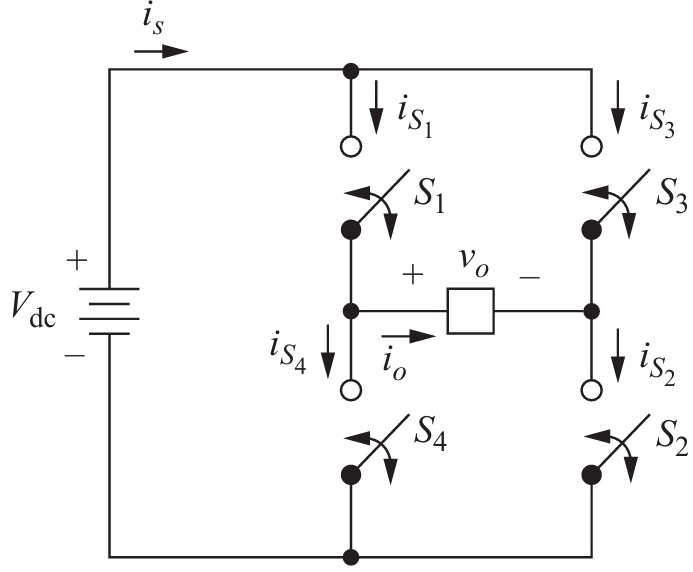
\includegraphics[scale=0.35]{gambar/square.jpg}
  % Keterangan gambar yang diinputkan
  \caption{Rangkaian inverter \emph{full bridge}}
  % Label referensi dari gambar yang diinputkan
  \label{fig:Inverter1}
\end{figure}

\begin{figure}[htbp] \centering
  % Nama dari file gambar yang diinputkan
  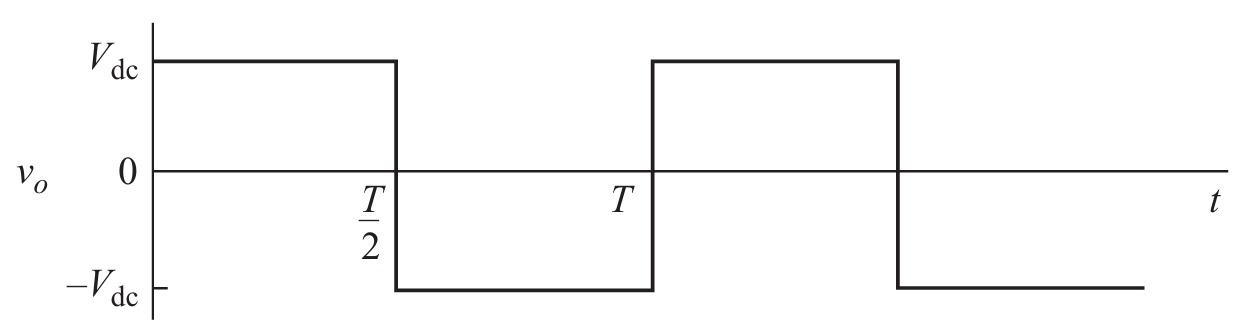
\includegraphics[scale=0.40]{gambar/square_wave.jpg}
  % Keterangan gambar yang diinputkan
  \caption{Tegangan keluaran inverter}
  % Label referensi dari gambar yang diinputkan
  \label{fig:Inverter}
\end{figure}

Pada Gambar~\ref{fig:Inverter} ditunjukkan tegangan keluaran inverter berbentuk
gelombang kotak (\emph{square wave}) dengan amplitudo $\pm V_{dc}$. Asumsikan $S_{\text{1}}$ dan $S_{\text{2}}$ tertutup pada $t=0$. 
Maka diperoleh persamaan arus pada beban dalam kondisi \emph{steady state} adalah sebagai berikut
\parencite{hart}.

\begin{equation}
i_o(t) =
\begin{cases}
\displaystyle \frac{V_{dc}}{R} + \left( I_{\min} - \frac{V_{dc}}{R} \right) e^{-t/\tau} & \text{untuk } 0 < t < \frac{T}{2} \\
\\
\displaystyle -\frac{V_{dc}}{R} + \left( I_{\max} + \frac{V_{dc}}{R} \right) e^{-(t - T/2)/\tau} & \text{untuk } \frac{T}{2} < t < T
\end{cases}
\end{equation}

Setelah itu dengan menggunakan analisis fourier, maka diperoleh persamaan tegangan
keluaran dari inverter yaitu.

\begin{equation}
    v_o(t) = \sum_{\substack{n \\ \text{odd}}} \frac{4V_{dc}}{n\pi} \sin(n \omega_0 t)
\end{equation}

Salah satu teknik penyaklaran dalam inverter satu fasa adalah dengan menggunakan
\emph{Pulse Width Modulation} (PWM). Dimana pada saat menggunakan PWM maka dapat
mengurangi total harmonisa pada arus beban. Dalam teknik PWM, amplitudo tegangan yang
dikeluarkan dapat diatur dengan sinyal gelombang yang termodulasi. Teknik ini memerlukan
sinyal referensi (sinyal yang termodulasi) yang berupa sinyal sinusoidal, dan sinyal
\emph{carrier}, yaitu sinyal triangular yang mengkontrol frekuensi \emph{switching}
\parencite{hart}. Salah satu teknik dalam PWM adalah \emph{bipolar switching}
\parencite{bipolar}. Pada Gambar~\ref{fig:bipolar-pwm} ditunjukkan bentuk gelombang
\emph{bipolar pulse width modulation}.

\begin{figure}[htbp] \centering
  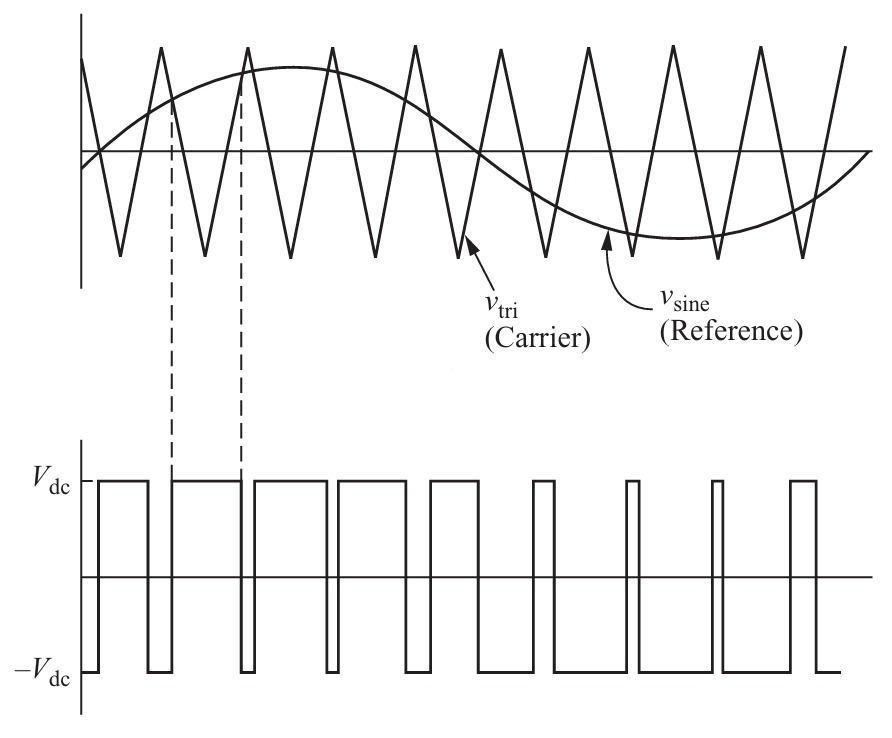
\includegraphics[scale=0.40]{gambar/inverter3.jpg}
  \caption{Bipolar \emph{pulse width modulation}}
  \label{fig:bipolar-pwm}
\end{figure}

\[
\begin{aligned}
v_o &= +V_{dc} \quad \text{saat } v_{\text{sine}} > v_{\text{tri}} \\
v_o &= -V_{dc} \quad \text{saat } v_{\text{sine}} < v_{\text{tri}}
\end{aligned}
\]

\[
\begin{aligned}
S_1 \text{ dan } S_2 \text{ ON ketika } v_{\text{sine}} > v_{\text{tri}} \quad &\left( v_o = +V_{dc} \right) \\
S_3 \text{ dan } S_4 \text{ ON ketika } v_{\text{sine}} < v_{\text{tri}} \quad &\left( v_o = -V_{dc} \right)
\end{aligned}
\]

\subsection{Karakteristik Pompa Air}
Pompa merupakan perangkat yang berfungsi untuk memindahkan cairan dari satu lokasi ke
lokasi lainnya dengan meningkatkan tekanan pada cairan tersebut. Pompa sanggup menaikkan
air dalam pipa vertikal sampai pada ketinggian di mana berat air dan gravitasi menahan
air untuk tidak naik lebih tinggi dari itu, ketinggian ini disebut \emph{head}.
Persamaan \emph{head} adalah sebagai berikut.
\begin{equation}
H_m = \frac{(P_d - P_s) \times 10}{\rho}
\end{equation} Pada Gambar~\ref{fig:Kurva} ditunjukkan kurva karakteristik kerja pompa.

\begin{figure}[htbp] \centering
  % Nama dari file gambar yang diinputkan
  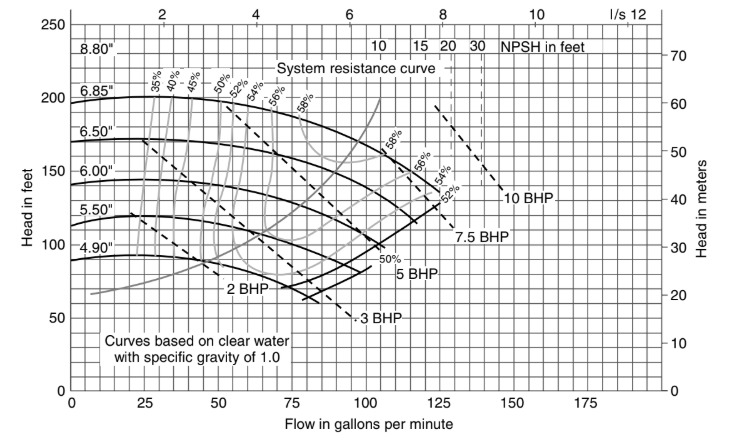
\includegraphics[scale=0.50]{gambar/kurva.jpg}
  % Keterangan gambar yang diinputkan
  \caption{Kurva karakteristik kerja pompa}
  % Label referensi dari gambar yang diinputkan
  \label{fig:Kurva}
\end{figure}

Pada kurva tersebut dapat dilihat hubungan antara debit dengan \emph{debit} dan kurva
tersebut menunjukkan titik potong yang merupakan titik kerja pompa. Kemudian, daya poros
motor (\(P_{Sh}\)) dapat dihitung dengan mengalikan torsi (\(\tau\)) yang dihasilkan
motor dengan kecepatan sudut (\(\omega\)) poros motor. Persamaannya adalah sebagai
berikut. Persamaan ini menunjukkan bahwa semakin besar torsi atau kecepatan putar motor,
maka daya yang disalurkan melalui poros motor juga akan semakin besar. Daya poros ini
merupakan salah satu komponen penting dalam perhitungan efisiensi motor maupun sistem
pompa secara keseluruhan \parencite{MANSOUR2025342}.

\begin{equation}
P_{Sh} = \tau \times \omega = \tau \times \frac{2\pi n}{60}
\end{equation}

Berdasarkan hukum afinitas, debit aliran $Q$ berbanding lurus dengan kecepatan putar
pompa. Artinya, jika kecepatan meningkat, maka debit aliran juga meningkat secara
proporsional.

\begin{equation}
Q_2 = Q_1 \times \left( \frac{N_2}{N_1} \right)
\end{equation}

\emph{Head} $H$ berbanding lurus dengan kuadrat dari perubahan kecepatan pompa. Artinya,
peningkatan kecepatan putar akan menaikkan head secara eksponensial.
\begin{equation}
H_2 = H_1 \times \left( \frac{N_2}{N_1} \right)^2
\end{equation}

Daya $P$ yang dibutuhkan oleh pompa berbanding lurus dengan pangkat tiga dari kecepatan.
Oleh karena itu, sedikit peningkatan kecepatan akan menyebabkan kenaikan daya yang cukup
signifikan.
\begin{equation}
P_2 = P_1 \times \left( \frac{N_2}{N_1} \right)^3
\end{equation}

Daya hidraulik yang dihasilkan oleh pompa $P_{\text{H}}$ bergantung pada debit aliran,
densitas fluida, percepatan gravitasi, dan \emph{H} (tekanan fluida). Persamaan untuk
menghitung daya hidraulik adalah sebagai berikut
\begin{equation}
P_H (\text{kW}) = \frac{Q \times \delta \times g \times H}{3.6 \times 10^6}
\end{equation}

Daya listrik yang disuplai ke motor (\(P_M\)) dapat dihitung dengan persamaan berikut.
\begin{equation}
P_M = \frac{\sqrt{3} \times V \times I \times \cos\phi}{1000 \times \eta_e}
\end{equation}

Dapat disimpulkan bahwa tegangan $V$ memengaruhi kecepatan motor dan tekanan motor
\parencite{GIRDHAR200548}.


\subsection{Motor Induksi Satu Fasa}

Motor induksi satu fasa banyak digunakan dalam aplikasi rumah tangga karena strukturnya
yang sederhana, biaya yang rendah, dan daya tahan yang tinggi. Prinsip kerja motor
induksi satu fasa didasarkan pada medan magnet berputar yang dihasilkan oleh arus
bolak-balik di stator, yang kemudian menginduksi arus pada rotor dan menghasilkan torsi
putar. Kecepatan medan magnet berputar dalam motor induksi, atau dikenal sebagai
kecepatan sinkron $n_{\text{sync}}$, bergantung pada frekuensi sumber $f_{\text{e}}$,dan
jumlah kutub P dari motor. sebagaimana ditunjukkan Persamaan~\eqref{eq:Persamaandas}

\begin{equation}
\label{eq:Persamaandas}
n_{\text{sync}} = \frac{120 f_e}{P}
\end{equation}

Dalam praktiknya, kecepatan aktual motor $n_{\text{m}}$ akan selalu sedikit lebih lambat
dari $n_{\text{sync}}$, selisihnya dinyatakan sebagai slip \text{s}. Slip menggambarkan
rasio perbedaan antara kecepatan sinkron dan kecepatan rotor terhadap kecepatan sinkron,
sebagaimana ditunjukkan oleh Persamaan~\eqref{eq:perss}

\begin{equation}
\label{eq:perss}
s = \frac{n_{\text{sync}} - n_m}{n_{\text{sync}}} \times 100\%
\end{equation}

Salah satu metode umum untuk mengatur kecepatan motor induksi adalah dengan memodifikasi
slip. Hal ini dapat dicapai baik dengan menambahkan resistansi rotor atau dengan
mengatur tegangan terminal motor \parencite{chapman}. Pada motor induksi satu fasa,
metode pengaturan tegangan terminal lebih umum digunakan.Dengan menurunkan tegangan RMS
terminal $V_{\text{T}}$ kecepatan motor dapat dikurangi karena slip meningkat. Persamaan
torsi dari motor induksi ditunjukkan pada Persamaan~\eqref{eq:perstorsi}.

\begin{equation}
\label{eq:perstorsi}
\tau_{\text{ind}} = \frac{P_{AG}}{\omega_{\text{sync}}}
\end{equation}

\begin{equation}
\label{eq:perstor2}
\tau_{\text{ind}} = 
\frac{3V_{\text{TH}}^2 \cdot \frac{R_2}{s}}{
\omega_{\text{sync}} \left[ \left( R_{\text{TH}} + \frac{R_2}{s} \right)^2 + (X_{\text{TH}} + X_2)^2 \right]}
\end{equation}

Dari Persamaan~\eqref{eq:perstor2} terlihat bahwa torsi sebanding dengan kuadrat tegangan
terminal $V_{\text{TH}}$ \parencite{hart}. Oleh karena itu, penurunan tegangan RMS
secara langsung mengurangi torsi output motor. Ini menunjukkan bahwa pengaturan tegangan
terminal tidak hanya berdampak pada slip dan kecepatan motor, tetapi juga mempengaruhi
kemampuan motor untuk menghasilkan torsi. Dengan demikian, pendekatan pengaturan
kecepatan menggunakan pengendalian tegangan terminal dapat dilakukan.

\subsection{IGBT (\emph{Insulated Gate Bipolar Transistor})}

\emph{Insulated Gate Bipolar Transistor} (IGBT) merupakan komponen saklar daya
semikonduktor yang menggabungkan keunggulan dua perangkat, yaitu gerbang masukan
berbasis MOSFET dan kanal keluaran berbasis transistor bipolar (BJT). Berkat
kombinasi tersebut, IGBT dapat dikendalikan oleh tegangan pada gerbang layaknya
MOSFET, namun mampu menghantarkan arus besar dengan rugi konduksi yang rendah
layaknya BJT. Karakteristik ini menjadikan IGBT banyak digunakan sebagai saklar
daya pada rangkaian elektronika daya bertegangan tinggi \parencite{hart}.

Secara struktur, IGBT memiliki tiga terminal, yaitu \emph{gate} (G),
\emph{collector} (C), dan \emph{emitter} (E). Secara internal, IGBT dapat
dipandang sebagai sebuah MOSFET kanal-n yang menggerakkan transistor bipolar PNP.
Pengoperasiannya dikendalikan melalui tegangan gerbang--emitter ($V_{GE}$): ketika
$V_{GE}$ melampaui tegangan ambang (\emph{threshold voltage}), terbentuk kanal
konduksi sehingga arus mengalir dari \emph{collector} menuju \emph{emitter};
sebaliknya ketika $V_{GE}$ berada di bawah tegangan ambang, IGBT berada pada
kondisi \emph{off} dan memblokir aliran arus. Oleh karena masukannya berupa
gerbang yang terisolasi, daya yang dibutuhkan untuk mengendalikan IGBT sangat
kecil.

IGBT bekerja dalam dua mode utama, yaitu mode \emph{on} (saturasi) dan mode
\emph{off} (\emph{cut-off}). Pemberian tegangan gerbang--emitter ($V_{GE}$) yang
positif memicu terbentuknya kanal-n pada lapisan p-\emph{base}, sehingga elektron
dapat mengalir dari \emph{emitter} menuju lapisan \emph{drift} n$^-$. Aliran
elektron tersebut kemudian menginjeksi \emph{hole} dari lapisan kolektor p$^+$ ke
daerah \emph{drift}, sehingga arus kolektor--emitter yang terbentuk merupakan
gabungan pembawa muatan mayoritas (\emph{hole}) dan minoritas (elektron). Ketika
$V_{GE}$ telah melampaui tegangan ambang ($V_{GE(th)}$), IGBT mulai berkonduksi
dan masuk ke kondisi \emph{on} (saturasi) sehingga arus mengalir dari
\emph{collector} menuju \emph{emitter}. Sebaliknya, apabila $V_{GE}$ diturunkan
hingga nol atau bernilai negatif, kanal-n akan hilang dan perangkat kembali ke
kondisi \emph{off} (\emph{cut-off}) yang menghentikan aliran arus kolektor
\parencite{hart}. Struktur dan simbol IGBT ditunjukkan pada
Gambar~\ref{fig:igbt}.

\begin{figure}[htbp] \centering
  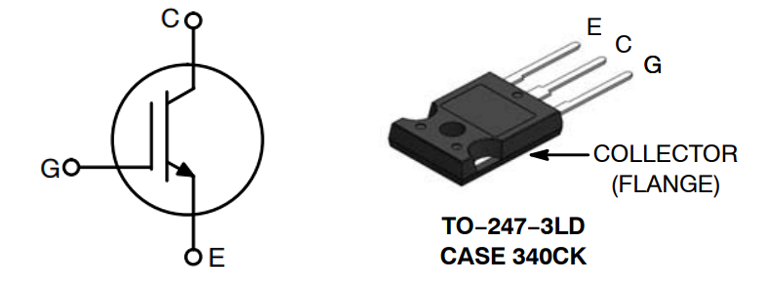
\includegraphics[width=0.55\linewidth]{gambar/igbt.png}
  \caption{Struktur dan simbol IGBT}
  \label{fig:igbt}
\end{figure}

Beberapa karakteristik utama IGBT adalah sebagai berikut \parencite{hart}.
\begin{enumerate}
    \item \textbf{Impedansi masukan tinggi (\emph{high input impedance}).}
    Gerbang IGBT yang terisolasi menjadikannya dikendalikan oleh tegangan dengan
    kebutuhan arus dan daya penggerak yang sangat kecil, serupa dengan MOSFET.
    \item \textbf{Kecepatan pensaklaran.} Kecepatan \emph{switching} IGBT lebih
    lambat dibandingkan MOSFET, tetapi masih tergolong cepat sehingga tetap sesuai
    untuk aplikasi pensaklaran pada frekuensi menengah hingga tinggi.
    \item \textbf{Tegangan jatuh konduksi rendah (\emph{low on-state voltage}).}
    IGBT memiliki tegangan jatuh \emph{collector--emitter} pada kondisi \emph{on}
    ($V_{CE(sat)}$) yang rendah walaupun memiliki peringkat tegangan dadal
    (\emph{breakdown voltage}) yang tinggi, sehingga rugi konduksinya tetap kecil
    pada tegangan kerja yang tinggi.
\end{enumerate}

Karakteristik keluaran IGBT ditunjukkan pada Gambar~\ref{fig:karakteristik-igbt},
yang menggambarkan hubungan antara arus kolektor ($I_C$) terhadap tegangan
kolektor--emitter ($V_{CE}$) untuk beberapa nilai tegangan gerbang--emitter
($V_{GE}$).

\begin{figure}[htbp] \centering
  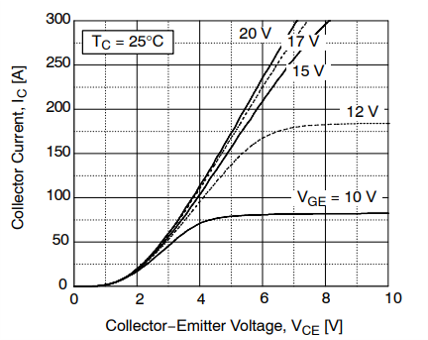
\includegraphics[width=0.6\linewidth]{gambar/karakteristik_igbt.png}
  \caption{Karakteristik keluaran IGBT ($I_C$ terhadap $V_{CE}$)}
  \label{fig:karakteristik-igbt}
\end{figure}

Dari grafik tersebut terlihat bahwa setiap kurva berlaku untuk satu nilai $V_{GE}$
yang berada di atas tegangan ambang, dan terdapat dua daerah kerja utama. Pada
daerah dengan $V_{CE}$ kecil (daerah aktif), arus kolektor meningkat tajam seiring
kenaikan $V_{CE}$; daerah ini merupakan wilayah transisi yang dilewati IGBT saat
proses pensaklaran. Setelah $V_{CE}$ cukup besar, kurva memasuki daerah saturasi,
yaitu arus kolektor cenderung mendatar (jenuh) dan besarnya ditentukan terutama
oleh nilai $V_{GE}$, bukan lagi oleh $V_{CE}$. Semakin besar $V_{GE}$, semakin
tinggi pula arus kolektor yang dapat dihantarkan, sehingga keluarga kurva bergeser
ke atas. Ketika difungsikan sebagai saklar daya, IGBT dioperasikan berpindah di
antara dua titik ekstrem, yaitu kondisi \emph{cut-off} ($V_{GE} < V_{GE(th)}$
dengan $I_C \approx 0$) dan daerah saturasi yang memiliki tegangan jatuh
$V_{CE(sat)}$ kecil, sehingga rugi konduksi pada kondisi \emph{on} menjadi minimal
\parencite{hart}.

Kombinasi impedansi masukan yang tinggi, kecepatan pensaklaran yang memadai, serta
rugi konduksi yang rendah pada tegangan tinggi inilah yang menjadikan IGBT pilihan
yang tepat sebagai saklar daya pada rangkaian PWM AC \emph{chopper} yang bekerja
pada tegangan jala-jala 220 V.

\subsection{Rangkaian PWM AC \emph{Chopper}}

PWM AC \emph{chopper} merupakan metode pengaturan tegangan AC menggunakan \emph{pulse
width modulation}. Sebagai pengatur tegangan pada motor, PWM AC chopper mampu memberikan
kontrol tegangan yang lebih linear saat \emph{starting}, menghasilkan torsi awal yang
lebih halus. Selain itu, pengoperasian pada frekuensi \emph{switching} tinggi
memungkinkan bentuk gelombang arus yang lebih mendekati sinusoidal dibandingkan dengan
pengontrol berbasis thyristor \parencite{pwmacchop2}. Rangkaian ini dikendalikan
berdasarkan interval waktu $T_{\text{on}}$ dan $T_{\text{off}}$, yang menentukan
karakteristik pensaklaran. Tegangan pada beban induktif selanjutnya dirumuskan dalam
Persamaan~\eqref{eq:Tegangan Beban}.

\begin{equation}
% Label referensi dari persamaan yang dibuat
\label{eq:Duty Ratio}
D = \frac{T_{\text{on}}}{T_s} = \frac{T_{\text{on}}}{T_{\text{on}} + T_{\text{off}}}
\end{equation}

\begin{equation}
% Label referensi dari persamaan yang dibuat
\label{eq:Tegangan Beban}
V_L(t) = D \cdot V_m \sin(\omega t)
\end{equation}
Susunan saklar pada rangkaian PWM AC \emph{chopper} ditunjukkan pada Gambar~\ref{fig:Saklar PWM AC}.

\begin{figure}[htbp] \centering
  % Nama dari file gambar yang diinputkan
  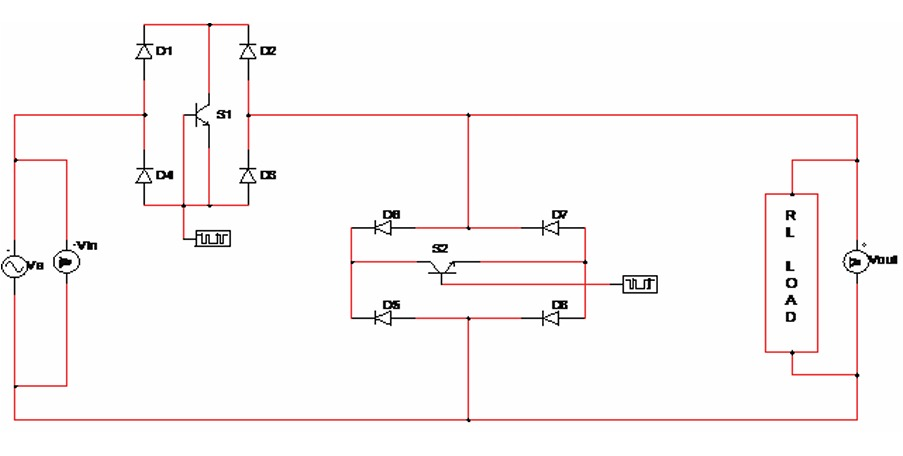
\includegraphics[scale=0.40]{gambar/pwm_ac_chop.jpg}
  % Keterangan gambar yang diinputkan
  \caption{Susunan saklar pada rangkaian PWM AC \emph{chopper}}
  % Label referensi dari gambar yang diinputkan
  \label{fig:Saklar PWM AC}
\end{figure}

Saklar S1 berfungsi sebagai saklar utama PWM yang mengatur waktu pada saat beban
menerima tegangan. Saklar S2 dan dioda berfungsi sebagai jalur bebas \emph{freewheeling}
saat S1 dimatikan, untuk menjaga arus tetap kontinu dan mencegah gangguan pada beban
induktif. Dengan mengubah rasio ON dan OFF \emph{duty cycle} dari S1, tegangan rata-rata
(RMS) yang diterima beban bisa diatur \parencite{pwmacchop}.
Cara kerja rangkaian AC chopper disajikan pada Tabel~\ref{tab:ac_chopper_operation}.

\begin{table}[H]
\caption{Cara kerja rangkaian}
\centering
\renewcommand{\arraystretch}{1.6}
\begin{tabularx}{\linewidth}{|
  >{\centering\arraybackslash}X|
  >{\centering\arraybackslash}X|
  >{\centering\arraybackslash}X|}
\hline
\textbf{Titik Kerja} & \textbf{ON} & \textbf{OFF} \\
\hline
Tegangan Setengah Fasa Positif & D1, S1, D3 \newline Aktif & D5, S2, D7 \newline Aktif \\
\hline
Tegangan Setengah Fasa Negatif & D2, S1, D4 \newline Aktif & D6, S2, D8 \newline Aktif \\
\hline
\end{tabularx}
\label{tab:ac_chopper_operation}
\end{table}

Untuk memahami cara kerja rangkaian secara lebih rinci, operasi PWM AC
\emph{chopper} pada motor induksi satu fasa dapat ditinjau berdasarkan arah
arus dan polaritas tegangan beban. Berdasarkan hal tersebut, terdapat enam mode
kerja yang terbagi menjadi tiga mode pada setengah siklus positif (Mode~1--3)
dan tiga mode pada setengah siklus negatif (Mode~4--6), sebagaimana ditunjukkan
pada Gambar~\ref{fig:mode-pwm-chopper} \parencite{6523243}.

\begin{figure}[htbp]
  \centering
  \begin{subfigure}{0.46\textwidth}\centering
    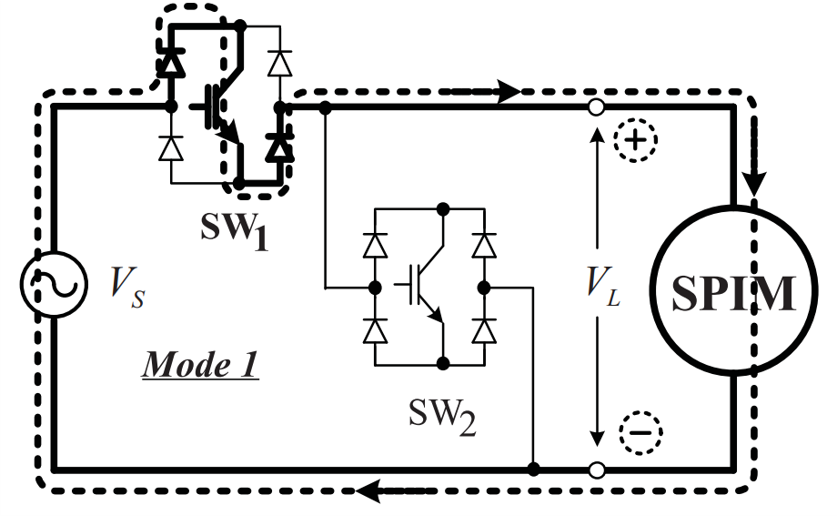
\includegraphics[width=\linewidth]{gambar/mode1.png}
    \caption{}\label{fig:mode1}
  \end{subfigure}\hfill
  \begin{subfigure}{0.46\textwidth}\centering
    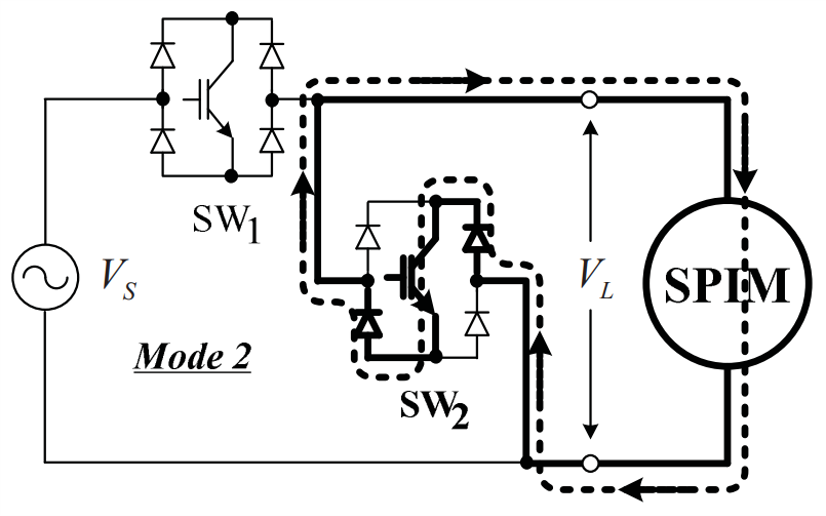
\includegraphics[width=\linewidth]{gambar/mode2.png}
    \caption{}\label{fig:mode2}
  \end{subfigure}

  \par\medskip
  \begin{subfigure}{0.46\textwidth}\centering
    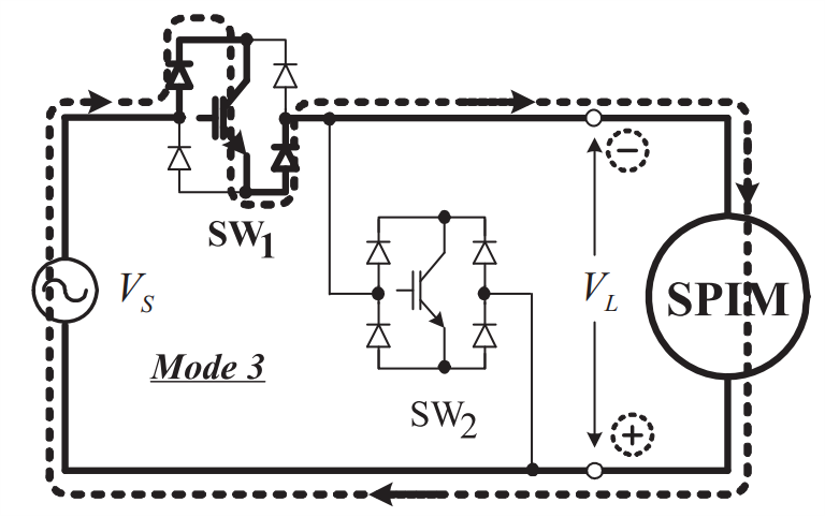
\includegraphics[width=\linewidth]{gambar/mode3.png}
    \caption{}\label{fig:mode3}
  \end{subfigure}\hfill
  \begin{subfigure}{0.46\textwidth}\centering
    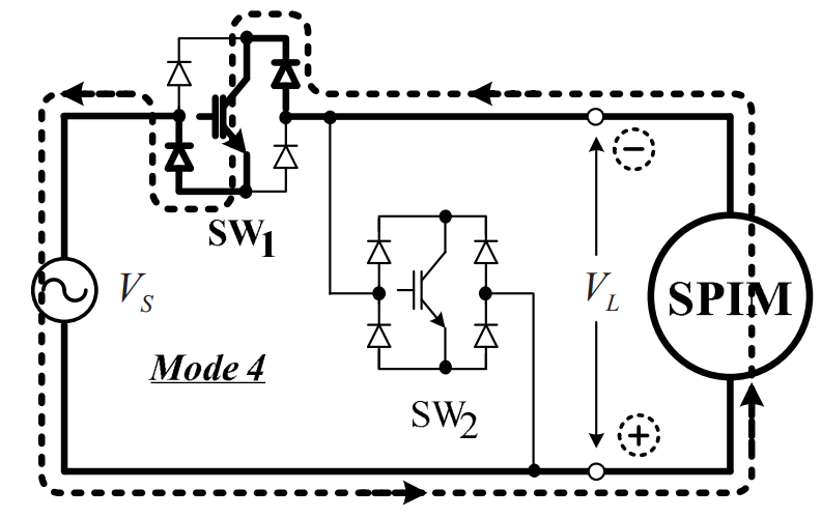
\includegraphics[width=\linewidth]{gambar/mode4.png}
    \caption{}\label{fig:mode4}
  \end{subfigure}

  \par\medskip
  \begin{subfigure}{0.46\textwidth}\centering
    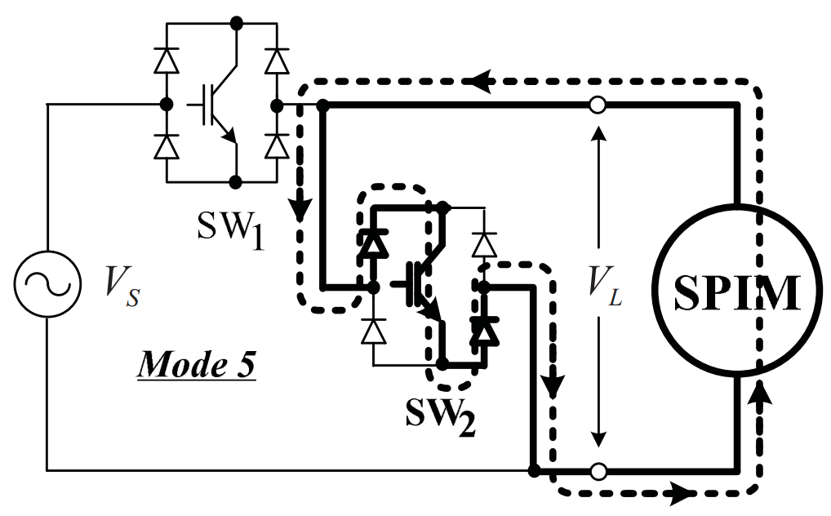
\includegraphics[width=\linewidth]{gambar/mode5.png}
    \caption{}\label{fig:mode5}
  \end{subfigure}\hfill
  \begin{subfigure}{0.46\textwidth}\centering
    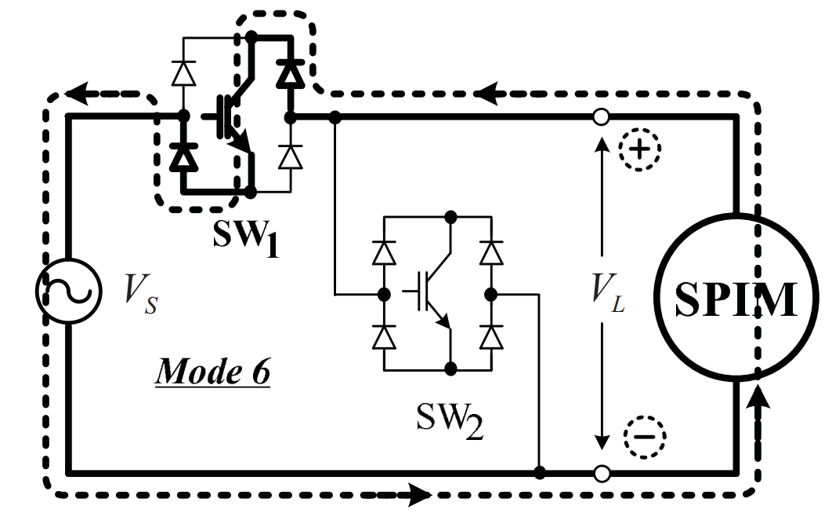
\includegraphics[width=\linewidth]{gambar/mode6.png}
    \caption{}\label{fig:mode6}
  \end{subfigure}
  \caption{Mode operasi rangkaian PWM AC \emph{chopper} pada motor induksi
  satu fasa: (a) Mode~1, (b) Mode~2, (c) Mode~3, (d) Mode~4, (e) Mode~5, dan
  (f) Mode~6}
  \label{fig:mode-pwm-chopper}
\end{figure}

Penjelasan masing-masing mode kerja tersebut adalah sebagai berikut.
\begin{itemize}[nolistsep]
  \item Mode~1 (\emph{powering}). SW$_1$ dihidupkan dan SW$_2$
        dimatikan. Arus mengalir dari sumber ($V_S$) melalui SW$_1$ menuju motor
        sehingga arus motor bernilai positif. Tegangan pada motor $V_L = +V_S$
        dan daya bernilai positif, yang berarti motor menyerap daya dari sumber.
  \item Mode~2 (\emph{freewheeling}). SW$_1$ dimatikan dan SW$_2$
        dihidupkan. SW$_2$ memungkinkan arus bersirkulasi pada motor tanpa kembali
        ke sumber sehingga tegangan motor menjadi nol. Arus tetap positif mengalir
        melalui SW$_2$, dioda, dan motor, sehingga arus motor menurun.
  \item Mode~3 (\emph{regenerative}). SW$_1$ dihidupkan dan SW$_2$
        dimatikan. Arus mengalir pada arah yang sama seperti Mode~1, tetapi
        polaritas tegangan motor berlawanan. Daya bernilai negatif dan
        dikembalikan ke sumber.
  \item Mode~4 (\emph{powering}). SW$_1$ dihidupkan dan SW$_2$
        dimatikan. Arus mengalir dari sumber ($V_S$) melalui motor menuju SW$_1$
        sehingga arus motor bernilai negatif. Tegangan pada motor $V_L = -V_S$ dan
        daya bernilai positif, yang berarti motor menyerap daya dari sumber.
  \item Mode~5 (\emph{freewheeling}). SW$_1$ dimatikan dan SW$_2$
        dihidupkan. SW$_2$ memungkinkan arus bersirkulasi pada motor tanpa kembali
        ke sumber sehingga tegangan motor menjadi nol. Arus tetap negatif mengalir
        melalui SW$_2$, dioda, dan motor, sehingga arus motor menurun.
  \item Mode~6 (\emph{regenerative}). SW$_1$ dihidupkan dan SW$_2$
        dimatikan. Arus mengalir pada arah yang sama seperti Mode~4, tetapi
        polaritas tegangan motor berlawanan. Daya bernilai negatif dan
        dikembalikan ke sumber.
\end{itemize}

\subsection{Kontrol \emph{Neural Network}}
\emph{Neural Network} atau jaringan saraf tiruan merupakan sistem komputasi yang
dikembangkan dengan meniru cara kerja otak manusia. Struktu dasar dari \emph{multilayer
perceptron} (MLP) NN dapat dilihat pada Gambar~\ref{fig:NN}. $x_{\text{1}}$-$x_{\text{2}}$
adalah \emph{input} sedangkan $y$ adalah \emph{output}. Terdapat tiga buah \emph{layer}
yaitu \emph{input layer}, \emph{hidden layer}, dan \emph{output layer} \parencite{ann}.

\begin{figure}[htbp] \centering
  % Nama dari file gambar yang diinputkan
  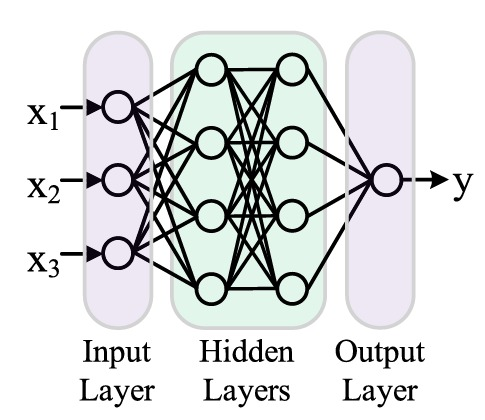
\includegraphics[scale=0.50]{gambar/nn.jpg}
  % Keterangan gambar yang diinputkan
  \caption{Struktur MPL NN}
  % Label referensi dari gambar yang diinputkan
  \label{fig:NN}
\end{figure}

Input skalar $p$ ditransmisikan melalui suatu koneksi yang mengalikan besarannya dengan
bobot skalar $w$, sehingga membentuk hasil kali $wp$, yang juga merupakan skalar. Dalam
hal ini, input berbobot $wp$ menjadi satu-satunya argumen dari fungsi transfer $f$, yang
menghasilkan output skalar $a$. Neuron pada sisi kanan memiliki suatu \textit{bias}
skalar, yaitu $b$.

\begin{equation}
a = f(wp + b)
\end{equation}
Struktur neuron sederhana diperlihatkan pada Gambar~\ref{fig:neuron}.

\begin{figure}[htbp] \centering
  % Nama dari file gambar yang diinputkan
  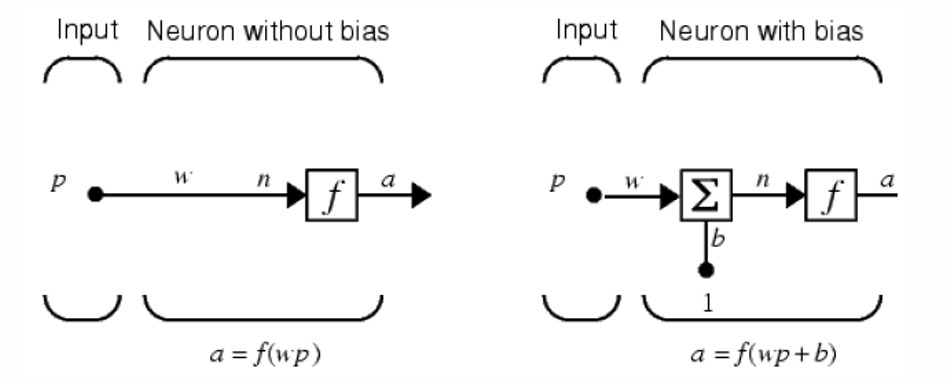
\includegraphics[scale=0.50]{gambar/simpleneuron.jpg}
  % Keterangan gambar yang diinputkan
  \caption{Neuron sederhana}
  % Label referensi dari gambar yang diinputkan
  \label{fig:neuron}
\end{figure}

Perceptron dilatih berdasarkan contoh-contoh perilaku yang diinginkan. Perilaku yang
diinginkan ini dapat dirangkum dalam bentuk pasangan input dan output sebagai berikut:

\[
(p_1, t_1),\ (p_2, t_2),\ \ldots,\ (p_q, t_q)
\]

di mana $p$ merupakan input ke jaringan dan $t$ adalah output yang benar (target) yang
sesuai. Tujuan dari pelatihan adalah untuk meminimalkan kesalahan $e$, yang merupakan
selisih antara respons neuron $a$ dan vektor target $t$. \emph{Learning Rules} dari
perseptron adalah sebagai berikut.

\begin{align*}
\mathbf{e}(k) &= \mathbf{t}(k) - \mathbf{a}(k) \\
\mathbf{w}(k+1) &= \mathbf{w}(k) + \mathbf{e}(k)\,\mathbf{p}^T(k) \\
\mathbf{b}(k+1) &= \mathbf{b}(k) + \mathbf{e}(k)\,\mathbf{1}^T(k)
\end{align*}

\emph{Inference} merupakan tahap penggunaan model neural network yang telah dilatih
untuk menghasilkan \emph{output} berdasarkan \emph{input} baru. Pada fase ini, model
tidak lagi mempelajari parameter \emph{weights} dan \emph{bias}, tetapi hanya melakukan
perhitungan forward pass untuk memperoleh prediksi.
Proses \emph{learning} pada neural network ditunjukkan pada Gambar~\ref{fig:learning}.

\begin{figure}[htbp] \centering
  % Nama dari file gambar yang diinputkan
  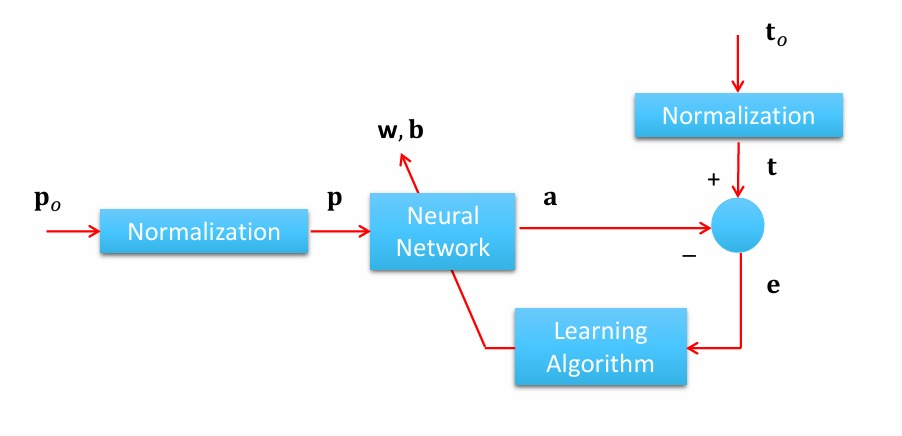
\includegraphics[scale=0.50]{gambar/learning.jpg}
  % Keterangan gambar yang diinputkan
  \caption{Proses \emph{learning}}
  % Label referensi dari gambar yang diinputkan
  \label{fig:learning}
\end{figure}

Proses pelatihan neural network terdiri dari dua fase utama yaitu \emph{forward
propagation} dan \emph{backpropagation}. \emph{Forward propagation} merupakan proses
dasar dalam jaringan saraf tiruan di mana data masukan melewati beberapa lapisan
jaringan untuk menghasilkan keluaran. Pada tahap ini, setiap lapisan akan melakukan
operasi matematis berupa perkalian bobot dan penambahan bias, lalu menerapkan fungsi
aktivasi.

\begin{align}
a^0 &= p \label{eq:input} \\
a^{m+1} &= f^{m+1}\left( \mathbf{w}^{m+1} a^m + b^{m+1} \right), \quad \text{untuk } m = 0, 1, \dots, M-1 \label{eq:recursive} \\
a &= a^M \label{eq:output}
\end{align}

\emph{Backpropagation} adalah algoritma pelatihan pada jaringan saraf tiruan yang bekerja
dengan menghitung kesalahan dari output dan menyebarkannya kembali ke lapisan sebelumnya
untuk memperbarui bobot. Proses ini dilakukan secara iteratif menggunakan metode
\emph{gradient descent} untuk meminimalkan kesalahan \parencite{backp}.

\begin{align}
s^M &= -2 \, \dot{\bm{F}}^M \left( \bm{n}^M \right) (t - \bm{a}) \label{eq:sM} \\
s^m &= \dot{\bm{F}}^m \left( \bm{n}^m \right) \left( \bm{w}^{m+1} \right)^T s^{m+1}, \quad \text{untuk } m = M-1, \ldots, 2, 1 \label{eq:sm}
\end{align}

\subsection{Metrik Evaluasi Model Regresi}
\label{subsec:metrik-evaluasi}

Kinerja model \emph{neural network} yang memprediksi nilai kontinu (regresi), perlu diukur menggunakan
metrik kesalahan (\emph{error}) yang sesuai. Untuk sejumlah $n$ data dengan nilai
aktual $y_i$ dan nilai prediksi $\hat{y}_i$, tiga metrik kesalahan yang paling
umum digunakan adalah \emph{Mean Absolute Error} (MAE), \emph{Mean Squared Error}
(MSE), dan \emph{Root Mean Squared Error} (RMSE) \parencite{hodson2022}.

\begin{align}
\text{MAE}  &= \frac{1}{n} \sum_{i=1}^{n} \left| y_i - \hat{y}_i \right| \label{eq:mae} \\
\text{MSE}  &= \frac{1}{n} \sum_{i=1}^{n} \left( y_i - \hat{y}_i \right)^2 \label{eq:mse} \\
\text{RMSE} &= \sqrt{ \frac{1}{n} \sum_{i=1}^{n} \left( y_i - \hat{y}_i \right)^2 } \label{eq:rmse}
\end{align}

  MAE merupakan rata-rata nilai mutlak selisih antara prediksi dan nilai aktual
  sehingga merepresentasikan besar kesalahan tipikal dan relatif
  \emph{robust} terhadap pencilan (\emph{outlier}). MSE merupakan rata-rata kuadrat
  selisih; karena selisih dikuadratkan, MSE menghukum kesalahan
besar secara lebih berat namun satuannya menjadi kuadrat dari satuan data
sehingga sulit ditafsirkan secara fisik. RMSE adalah akar kuadrat dari MSE,
sehingga memiliki satuan yang sama dengan data dan mencerminkan kesalahan
``standar'' atau tipikal model. Karena $\text{RMSE} = \sqrt{\text{MSE}}$, kedua
metrik ini membawa informasi yang sama; RMSE umumnya dilaporkan karena lebih
mudah ditafsirkan, sedangkan MSE lebih sering berperan sebagai fungsi rugi
(\emph{loss}) saat pelatihan.

Tidak ada metrik yang secara mutlak lebih unggul; pemilihannya bergantung pada
distribusi kesalahan model. RMSE optimal ketika kesalahan berdistribusi normal
(Gauss), sedangkan MAE optimal ketika kesalahan berdistribusi Laplace, karena
masing-masing meminimalkan fungsi rugi yang memaksimalkan \emph{likelihood} pada
distribusi tersebut \parencite{hodson2022}. Karakter distribusi kesalahan dapat
diperkirakan dari rasio RMSE/MAE: nilai mendekati $\sqrt{\pi/2}\approx 1{,}25$
mengindikasikan kesalahan bertipe Gauss, sedangkan nilai mendekati
$\sqrt{2}\approx 1{,}41$ mengindikasikan kesalahan bertipe Laplace yang lebih
runcing dan berekor tebal. Dengan demikian, melaporkan MAE dan RMSE bersama-sama
bermanfaat untuk mencirikan aspek kesalahan yang berbeda (kesalahan tipikal
versus sensitivitas terhadap kesalahan besar), selama keduanya tidak dianggap
sebagai bukti yang saling bebas.

Selain metrik kesalahan absolut di atas, kekuatan model regresi juga dinilai
menggunakan koefisien determinasi ($R^2$) yang bersifat tak berdimensi:

\begin{equation}
R^2 = 1 - \frac{\sum_{i=1}^{n} \left( y_i - \hat{y}_i \right)^2}
{\sum_{i=1}^{n} \left( y_i - \bar{y} \right)^2}
\label{eq:r2}
\end{equation}

dengan $\bar{y}$ adalah rata-rata nilai aktual. Koefisien $R^2$ menyatakan
proporsi keragaman data aktual yang mampu dijelaskan oleh model. Nilai $R^2 = 1$
menunjukkan kecocokan sempurna, sedangkan model yang buruk dapat menghasilkan
$R^2 < 0$ \parencite{avdeef2021}. Perlu dicatat bahwa terdapat beberapa definisi
$R^2$ (validasi model, kompensasi \emph{bias}, dan Pearson) yang dapat memberikan
nilai berbeda untuk data yang sama; pada penelitian ini digunakan definisi
validasi model seperti pada Persamaan~\eqref{eq:r2}, yang mengukur sebaran data
terhadap garis identitas $y = \hat{y}$ sehingga merepresentasikan kekuatan
hubungan langsung antara prediksi dan nilai aktual \parencite{avdeef2021}.

\subsection{STM32U545RE}

Mikrokontroler STM32U545RE merupakan mikrokontroler 32-bit berbasis inti ARM
Cortex-M33 yang mampu beroperasi pada frekuensi hingga 160 MHz. Mikrokontroler
ini dilengkapi beragam pewaktu (\emph{timer}), termasuk \emph{advanced-control
timer} yang mampu menghasilkan sepasang sinyal PWM komplementer beserta
\emph{dead time}, sehingga sesuai untuk pengendalian saklar daya.
STM32U545RE ditunjukkan pada Gambar~\ref{fig:stm}.

\begin{figure}[htbp] \centering
  % Nama dari file gambar yang diinputkan
  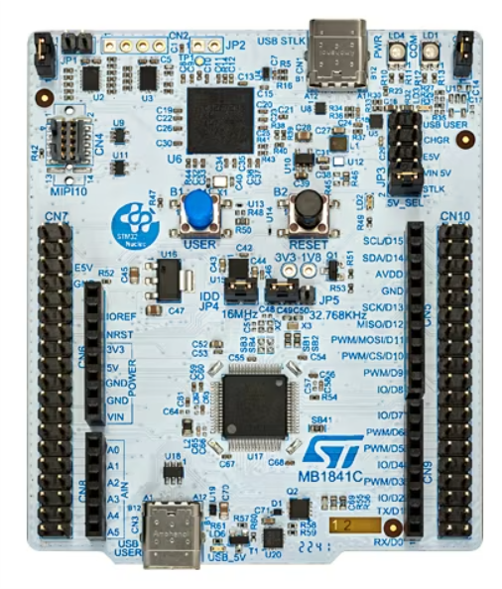
\includegraphics[scale=0.40]{gambar/stm32_u545.png}
  % Keterangan gambar yang diinputkan
  \caption{\emph{STM32U545RE}}
  % Label referensi dari gambar yang diinputkan
  \label{fig:stm}
\end{figure}

STM32U545RE juga dilengkapi \emph{Analog-to-Digital Converter} (ADC) beresolusi
hingga 14-bit dengan beberapa kanal masukan eksternal dan kecepatan konversi yang
tinggi. ADC ini mendukung mode \emph{single-shot} dan \emph{continuous
conversion}, serta fitur \emph{Direct Memory Access} (DMA) untuk transfer data
yang efisien tanpa membebani CPU \parencite{stm32}.

Spesifikasi utama STM32U545RE beserta pemanfaatannya pada sistem yang dirancang
dirangkum pada Tabel~\ref{tab:spek-stm32}.

\begin{table}[H]
\caption{Spesifikasi STM32U545RE dan pemanfaatannya pada sistem}
\centering
\renewcommand{\arraystretch}{1.4}
\begin{tabularx}{\linewidth}{|
  >{\raggedright\arraybackslash\hsize=0.8\hsize}X|
  >{\raggedright\arraybackslash\hsize=1.0\hsize}X|
  >{\raggedright\arraybackslash\hsize=1.2\hsize}X|}
\hline
\textbf{Fitur} & \textbf{Spesifikasi} & \textbf{Pemanfaatan pada sistem} \\
\hline
Inti prosesor & Arm Cortex-M33 32-bit, hingga 160 MHz, dengan FPU dan DSP &
Menjalankan algoritma kendali dan inferensi \emph{neural network} \\
\hline
Memori \emph{Flash} & 512 KB (dengan ECC) &
Menyimpan program dan parameter model \\
\hline
Memori SRAM & 274 KB &
Penyimpanan variabel selama program berjalan \\
\hline
ADC & Hingga 14-bit (dikonfigurasi 12-bit), kecepatan konversi tinggi &
Membaca tegangan keluaran sensor tekanan \\
\hline
\emph{Timer} TIM1 & \emph{Advanced-control timer} dengan PWM komplementer dan
\emph{dead time} & Membangkitkan sepasang sinyal PWM \emph{chopper} 5~kHz \\
\hline
USART1 & Komunikasi serial asinkron &
Pertukaran telemetri dan perintah dengan GUI pada PC \\
\hline
USART3 & Komunikasi serial (protokol Modbus RTU) &
Membaca sensor daya JSY (tegangan, arus, dan daya) \\
\hline
USB & 1 USB \emph{full-speed} (\emph{host/device}) &
Koneksi ke PC melalui \emph{Virtual COM Port} \\
\hline
GPIO & Hingga 82 jalur I/O, sebagian besar 5~V-\emph{tolerant} &
Jalur pin PWM, ADC, dan komunikasi \\
\hline
\end{tabularx}
\label{tab:spek-stm32}
\end{table}

\subsection{Sensor Tekanan Air}

Sensor tekanan air bekerja dengan mengubah tekanan fisik air melalui elemen seperti
diafragma, \emph{strain gauge}, atau kristal piezoelektrik menjadi sinyal listrik. Sinyal ini
kemudian diproses melalui amplifikasi, penyaringan \emph{noise}, dan konversi digital. Sensor
umumnya memiliki tiga pin, VCC (biasanya 5V), GND, dan pin sinyal (keluaran 0,5–4,5V).
Beberapa sensor memiliki \emph{output} berbasis nol (misalnya 0–5V) dan lainnya tidak (misalnya
1–5V), di mana pembacaan nol pada sensor non-basis nol menandakan kegagalan sensor
\parencite{waterpress}.

Secara lebih rinci, sebagian besar sensor tekanan air menggunakan diafragma
silikon yang berfungsi sebagai \emph{strain gauge}. Ketika air menekan
permukaan diafragma, elemen silikon melengkung sebanding dengan gaya tekanan
yang diterima. Lengkungan mekanis ini mengubah resistansi listrik
\emph{strain gauge}, yang selanjutnya dikonversi menjadi tegangan keluaran yang
proporsional terhadap tekanan. Pada pengukuran tekanan \emph{gauge}, sensor
dilengkapi jalur ventilasi agar tekanan atmosfer menjadi acuan pembacaan. Karena
media yang diukur berupa air, pemilihan bahan diafragma juga harus
mempertimbangkan ketahanan terhadap korosi serta kesesuaian dengan
karakteristik air (pH dan kandungan mineral) agar pembacaan tetap akurat dan
sensor tahan lama.

Salah satu contoh sensor tekanan air yang tersedia di pasaran adalah
\emph{DFRobot Gravity: Analog Water Pressure Sensor} (SEN0257). Sensor ini
bekerja pada tegangan 5~VDC dan menghasilkan tegangan keluaran analog
yang linear pada rentang 0,5--4,5~V untuk tekanan 0--1,6~MPa. Sensor
memiliki ulir G1/4 sehingga mudah dipasang pada instalasi perpipaan, tingkat
kedap air IP68, akurasi 0,5--1\% \emph{full scale}, serta waktu respons kurang
dari 2~ms \parencite{dfrobot_sen0257}. Karakteristik keluaran yang
linear memudahkan konversi tegangan sensor menjadi nilai tekanan.
Sensor tekanan air dan data pembacaannya ditunjukkan pada
Gambar~\ref{fig:water_sensor} dan Gambar~\ref{fig:water_data}.

\begin{figure}[htbp]
  \centering
  % Gambar kiri
  \begin{minipage}{0.48\textwidth}
    \centering
    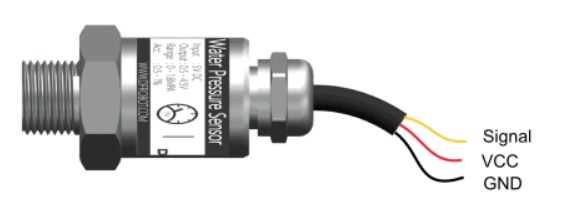
\includegraphics[scale=0.5]{gambar/sensor.jpg}
    \caption{\emph{Analog water pressure sensor}}
    \label{fig:water_sensor}
  \end{minipage}
  \hfill
  % Gambar kanan
  \begin{minipage}{0.48\textwidth}
    \centering
    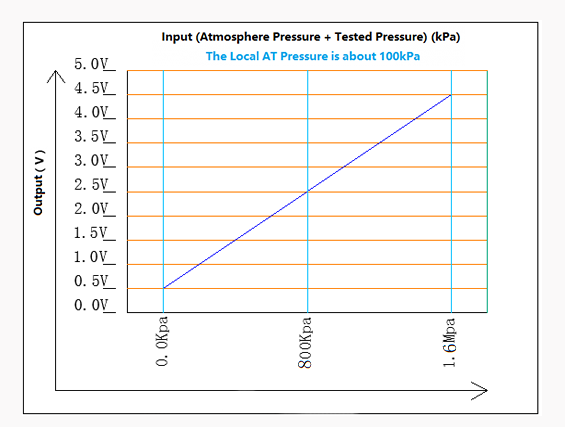
\includegraphics[scale=0.5]{gambar/data tekanan.png}
    \caption{\emph{Data pembacaan tekanan air}}
    \label{fig:water_data}
  \end{minipage}
\end{figure}

\subsection{Intensitas Cahaya (\emph{Exposure Value})}

\emph{Exposure Value} (EV) merupakan sebuah bilangan tunggal yang merepresentasikan
kombinasi pengaturan kamera dalam menangkap cahaya, sekaligus menjadi ukuran
kuantitatif terhadap intensitas cahaya (kecerahan) suatu adegan. Nilai EV
menyatukan pengaruh bukaan lensa (\emph{aperture}) dan kecepatan rana
(\emph{shutter speed}) ke dalam satu skala, sehingga tingkat pencahayaan yang sama
dapat dicapai oleh berbagai kombinasi keduanya \parencite{expval}.

Secara matematis, EV didefinisikan pada Persamaan~\eqref{eq:ev}.

\begin{equation}
\label{eq:ev}
EV = \log_2 \left( \frac{N^2}{t} \right)
\end{equation}

dengan $N$ adalah bilangan-f (\emph{f-number}) bukaan lensa dan $t$ adalah waktu
pencahayaan (kecepatan rana) dalam satuan detik. Definisi ini mengacu pada
sensitivitas ISO 100 sebagai acuan, yaitu nilai $EV = 0$ setara dengan pencahayaan
pada bukaan $f/1{,}0$ dengan rana selama satu detik.

Karena menggunakan basis logaritma dua, setiap kenaikan satu satuan EV setara
dengan penggandaan atau pengurangan setengah jumlah cahaya, yang dalam fotografi
dikenal sebagai satu \emph{stop}. Semakin tinggi nilai EV, semakin terang kondisi
pencahayaan (semakin sedikit cahaya yang perlu dikumpulkan); sebaliknya, nilai EV
yang rendah menandakan kondisi yang semakin gelap. Sebagai gambaran, kondisi
pencahayaan pada berbagai nilai EV (pada ISO 100) dirangkum pada
Tabel~\ref{tab:ev}.

\begin{table}[H]
\centering
\caption{Nilai \emph{exposure value} pada berbagai kondisi pencahayaan (ISO 100)}
\label{tab:ev}
\renewcommand{\arraystretch}{1.3}
\begin{tabularx}{\linewidth}{|c|>{\raggedright\arraybackslash}X|}
\hline
\textbf{EV (ISO 100)} & \textbf{Kondisi pencahayaan} \\
\hline
15 & Siang hari cerah, sinar matahari langsung (bayangan tegas) \\
\hline
14 & Siang hari dengan sinar matahari berkabut tipis \\
\hline
12 & Langit mendung atau berawan tebal \\
\hline
9--11 & Matahari terbenam dan cahaya lemah di luar ruangan \\
\hline
7--8 & Ruangan dengan pencahayaan terang \\
\hline
5--6 & Interior rumah pada malam hari \\
\hline
1--4 & Jalan pada malam hari dengan penerangan lampu \\
\hline
$\leq 0$ & Cahaya bulan dan kondisi sangat gelap \\
\hline
\end{tabularx}
\end{table}

Selain \emph{aperture} dan \emph{shutter speed}, tingkat pencahayaan akhir juga
dipengaruhi oleh sensitivitas ISO. Kenaikan nilai ISO memperbesar sensitivitas
sensor terhadap cahaya sehingga secara efektif menaikkan pencahayaan pada nilai EV
yang sama. Dengan demikian, konsep EV menjadi dasar dalam mengukur dan mengatur
intensitas cahaya secara kuantitatif \parencite{expval}. 

